\chapter{Parameter Calibrations}
\label{paramcalib}

\section{Stock returns}
\label{paramcalibx}
We use log differences on our monthly stock price data to obtain historical monthly rates of return. The Augmented Dickey-Fuller test strongly shows that the modified series is stationary at $1\%$ significance level.

\begin{figure}[h!]
	\centering
	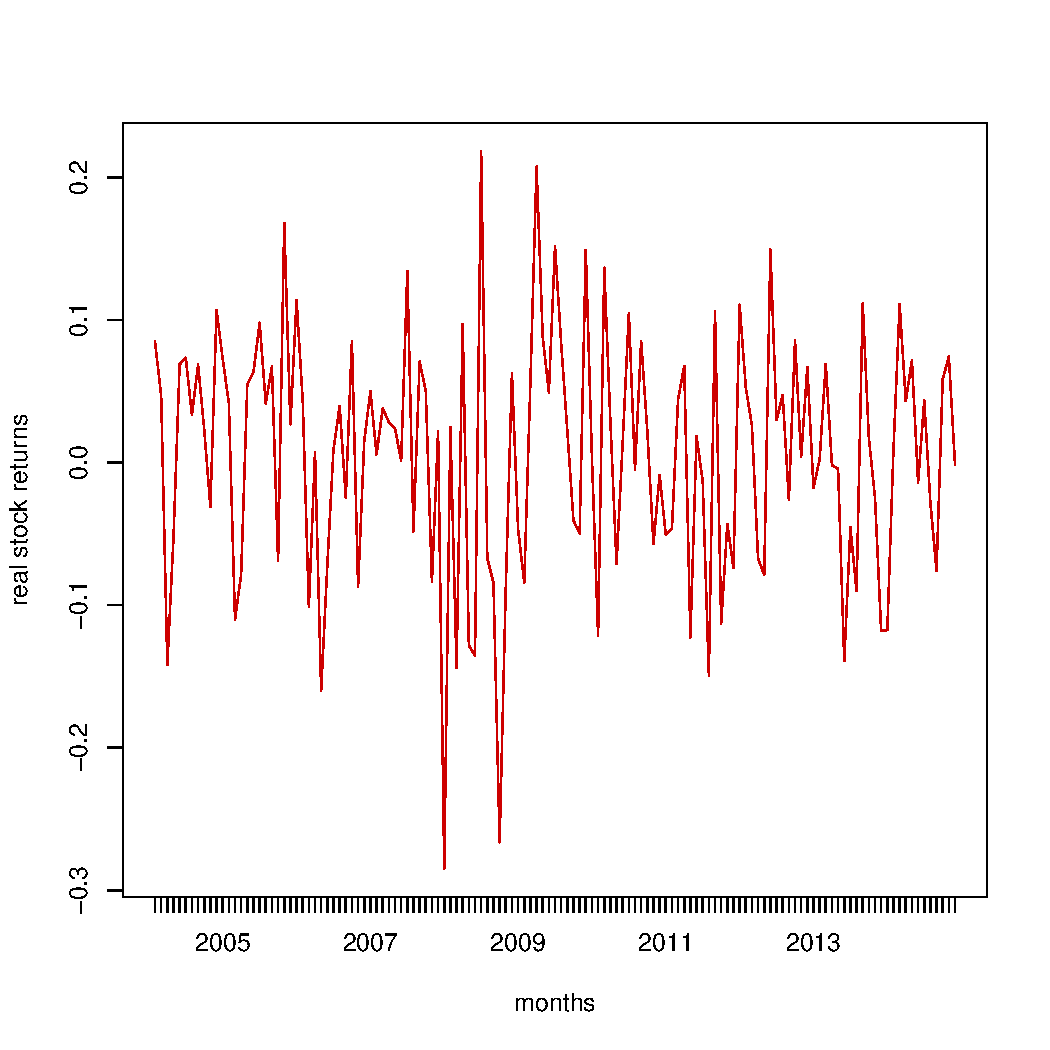
\includegraphics[scale=0.3]{figs/bistdiff.pdf}
	\caption{Historical monthly rates of return on stocks}
	\label{fig:bistdiff}
\end{figure}

We use Akaike Information Criterion to find the optimal lag order for ARIMA estimation --- $p=q=2$.

Performing ARIMA(2,0,2) estimation, we obtain the long-term forecasted monthly rate of return $\mu^S_{mon} = 0.541\%$ and volatility $\sigma^S_{mon} = 11.1\%$.

Finally, we annualize these values as follows:

\begin{equation}
	\mu_S = (1 + \mu^S_{mon})^{12} - 1= 6.69\%
\end{equation}

\begin{equation}
	\sigma_S = \sigma^S_{mon} \cdot \sqrt{12} = 38.44\%
\end{equation}

\section{Housing returns}
\label{paramcaliby}
Similarly, we log-differentiate monthly house prices to obtain growth rates. The house market collapse of 2008 brings large external shock, causing the Augmented Dickey-Fuller test to only find stationarity at $10\%$ significance level for 3 lags at most.

\begin{figure}[h!]
	\centering
	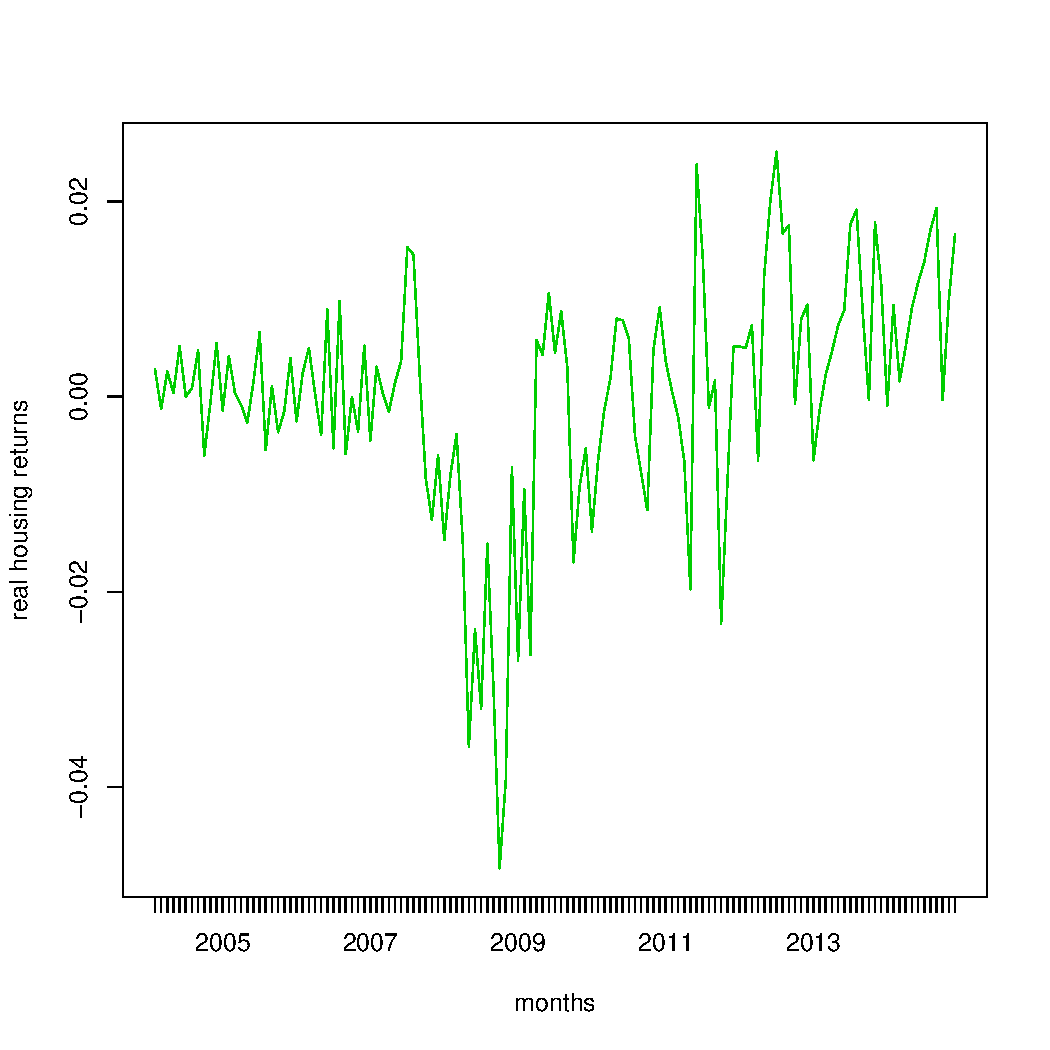
\includegraphics[scale=0.3]{figs/reidindiff.pdf}
	\caption{Historical monthly rates of return on housing}
	\label{fig:reidindiff}
\end{figure}

Again, using Akaike Information Criterion, we find $p=q=1$.

ARIMA(1,0,1) estimation provides long-term forecasts for monthly rate of return and volatility as $\mu^H_{mon} = 0.06\%$ and $\sigma^H_{mon} = 1.57\%$.

Annualization gives:

\begin{equation}
	\mu_H = (1 + \mu^H_{mon})^{12} - 1= 0.67\%
\end{equation}

\begin{equation}
	\sigma_H = \sigma^H_{mon} \cdot \sqrt{12} = 5.42 \%
\end{equation}


\section{Labor income volatility}
\label{paramcalibz}
The Augmented Dickey-Fuller test returns stationarity for up to 9 lags at $5\%$ significance level. 

\begin{figure}[h!]
	\centering
	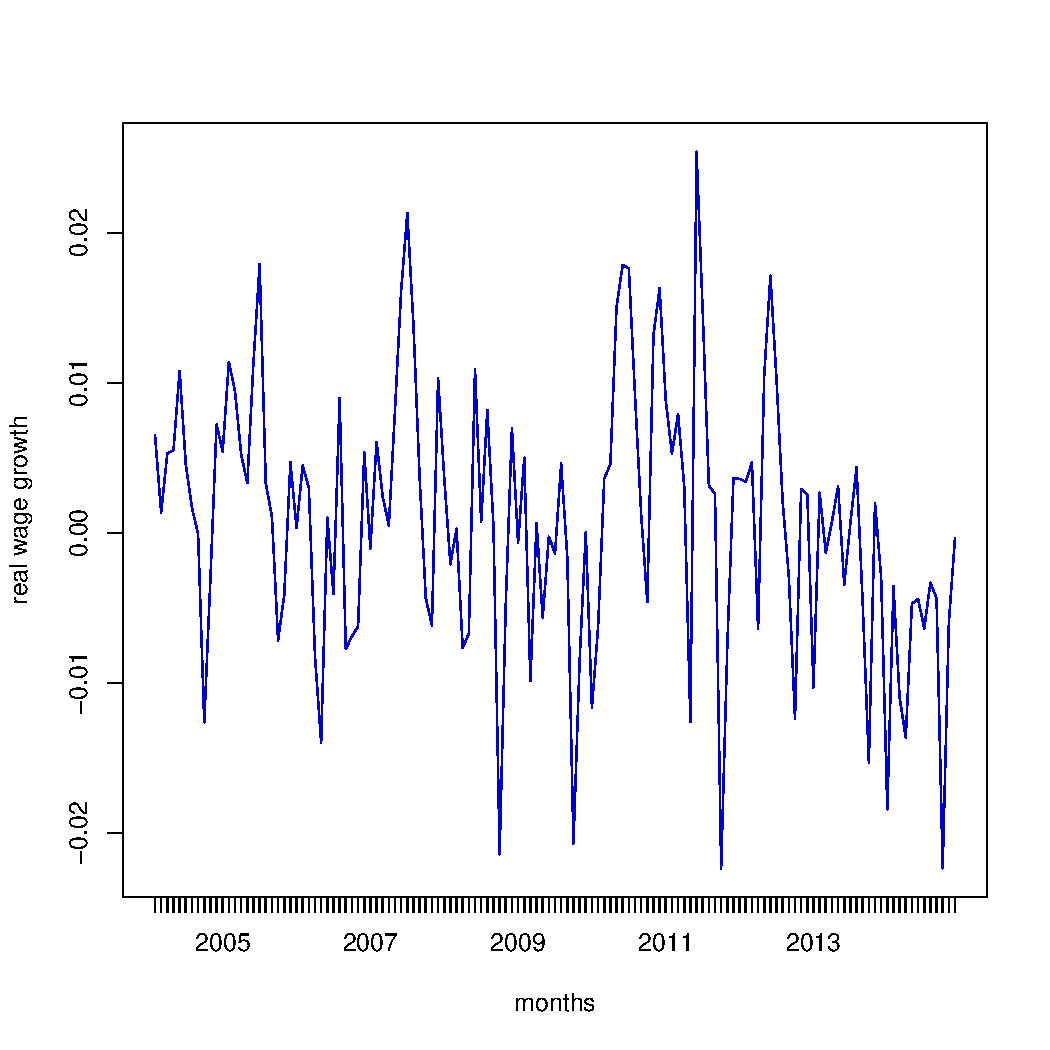
\includegraphics[scale=0.3]{figs/wagediff.pdf}
	\caption{Historical monthly wage growth rates}
	\label{fig:wagediff}
\end{figure}

Akaike Information Criterion suggests $p=5$ and $q=2$.

ARIMA(5,0,2) estimation gives monthly volatility $\sigma^L_{mon} = 1.04\%$, which annualizes as follows:

\begin{equation}
	\sigma_L = \sigma^L_{mon} \cdot \sqrt{12} = 3.59 \%
\end{equation}


\section{Wage regression results}
\label{paramcalibt}

The regressions of wage growth rates by age with kinks at 40 and 55, return the following coefficients.

\begin{table}[H]
	\centering
	\caption[]{Wage regression results by age}
	\begin{tabular}[c]{lccc}
		\hline
		&flat&moderate&steep\\
		\hline
		(intercept)&0.1\%&0.4\%&1.5\%\\
		d40&-0.7\%&3.3\%&0.7\%\\
		d55&1.4\%&0.9\%&-0.4\%\\
		\hline
	\end{tabular}
\end{table}

The growth rates can be calculated using these coefficients. Note that we have rounded the growth rates for the flat wages to $0$. Figure \ref{fig:heterwage} illustrates how the estimated rates fit the data:

\begin{figure}[h!]
	\centering
	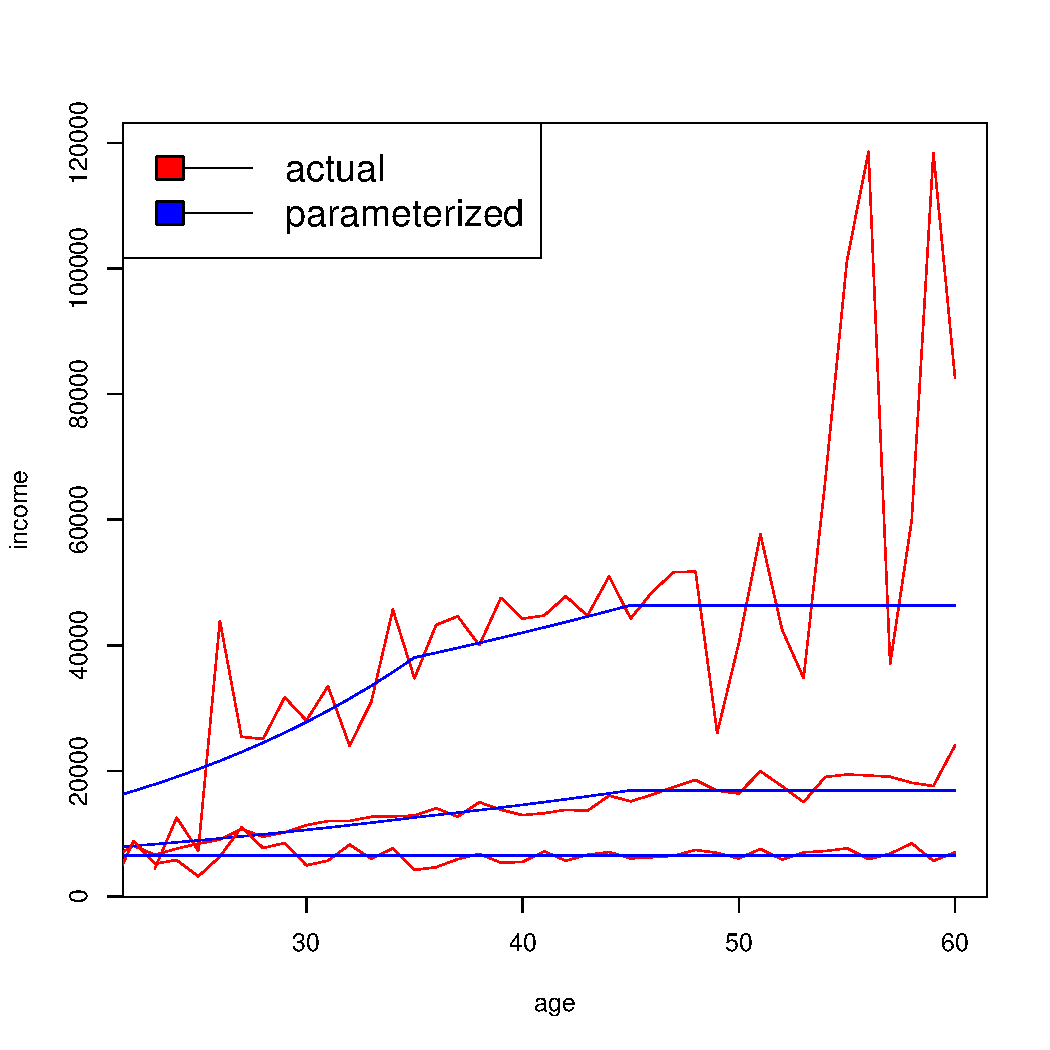
\includegraphics[scale=0.3]{figs/heterwage.pdf}
	\caption{Fitted values from wage regressions}
	\label{fig:heterwage}
\end{figure}


